%% REDO THE PLOTS

\section{Figures}

\subsection{\textit{Ex-ante} KPCA}
% EX ANTE
% scree ante
\begin{figure}[H]  
\centering
\includegraphics[width=12cm,height=8cm]{./Figures/scree_ante.eps}
\caption{\textit{ex-ante} KPCA: Normalized root-mean-squared reconstruction error for 1 epoch, and 32, 64, 128, 256, 512 dimensions. Lower is better.} 
\label{fig:scree_ante}
\end{figure}


% cos_dist_ante
\begin{figure}[H]  
\centering
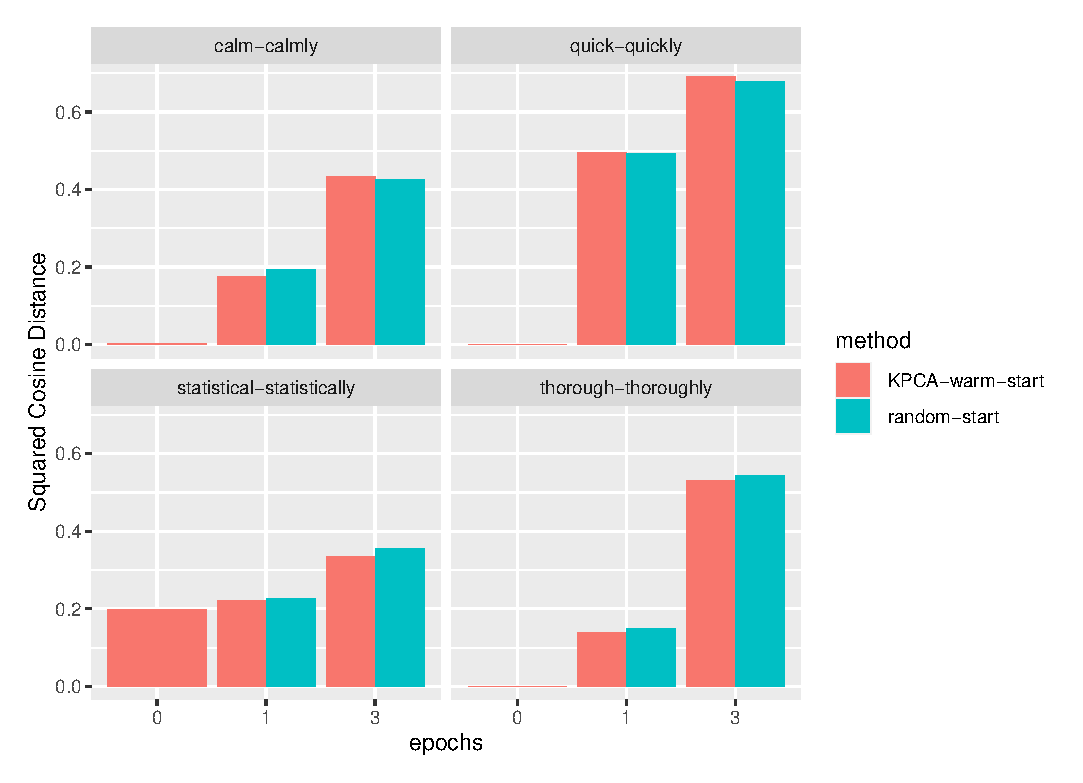
\includegraphics[width=12cm,height=9cm]{Figures/cos_dist_ante.eps}
\caption{\textit{ex-ante} KPCA: Squared cosine distance between \textbf{adjective-adverb pairs}, with KPCA-initialized (no further training, 1, 3 epochs) and random-initialized (1 and 3 epochs) word2vec. Lower is better.}
\label{fig:cos_dist_ante}
\end{figure}

% spearman
\begin{figure}[H]  
\centering
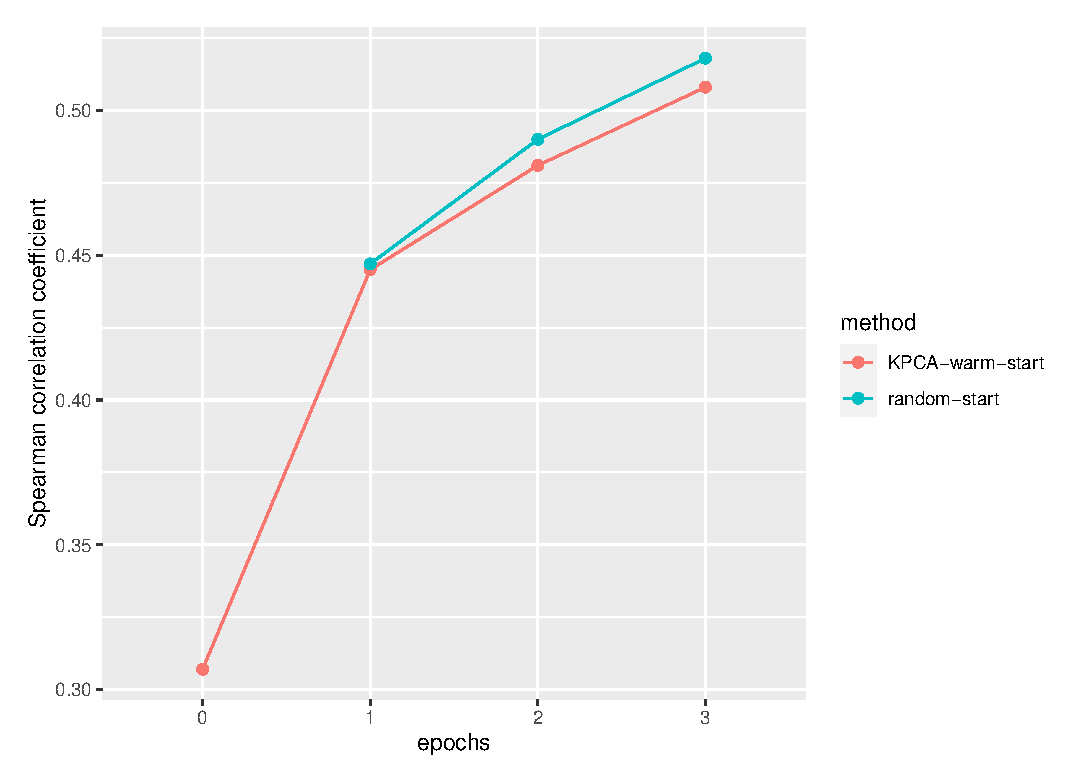
\includegraphics[width=14cm,height=10cm]{./Figures/spear_ante.eps}
\caption{\textit{ex-ante} KPCA: \textbf{Spearman correlation coefficient} of KPCA-initialized (no further training, 1, 3 epochs) and random-initialized (1 and 3 epochs) word2vec with state-of-the-art embeddings.} 
\label{fig:spear_ante}
\end{figure}





\subsection{\textit{Ex-post} KPCA}
% EX POST

% scree post
\begin{figure}[H]  
\centering
\includegraphics[width=12cm,height=8cm]{./Figures/scree_post.eps}
\caption{ \textit{ex-post} KPCA: Normalized root-mean-squared reconstruction error for 1, 2, 3 epochs, and 8, 16, 32, 64 dimensions. Lower is better.} 
\label{fig:scree_post}
\end{figure}

% cos_dist_post
\begin{figure}[H]  
\centering
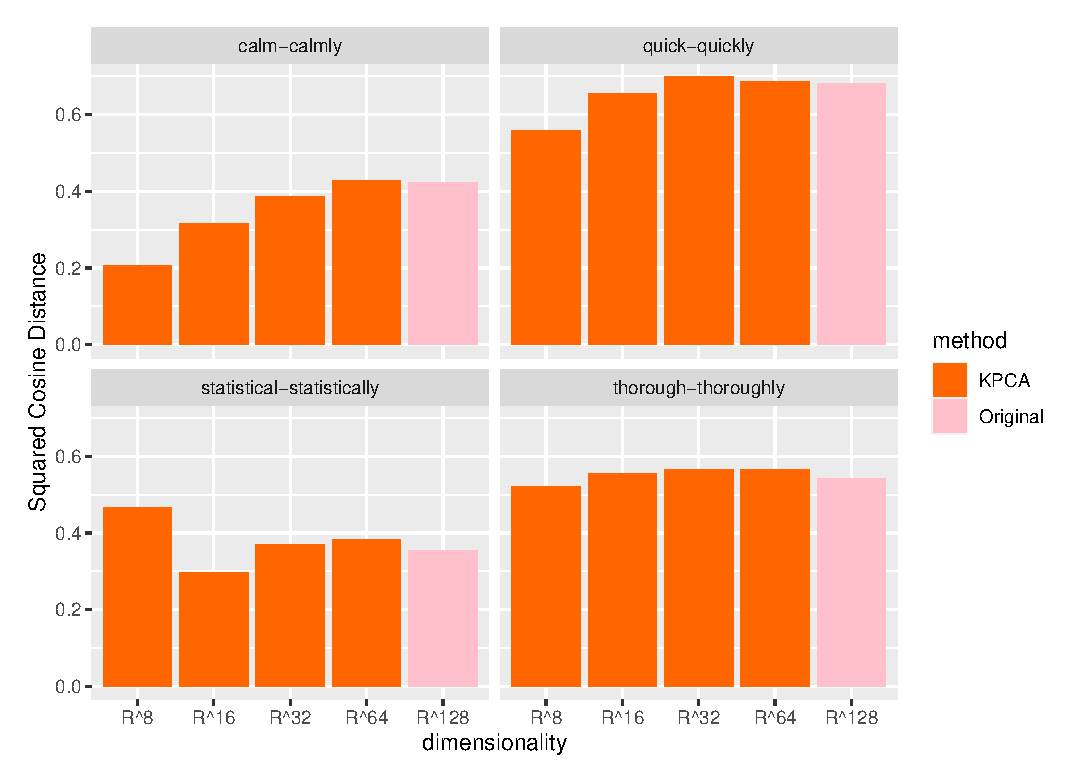
\includegraphics[width=12cm,height=9cm]{./Figures/cos_dist_post.eps}
\caption{ \textit{ex-post} KPCA: Squared cosine distance between adjective-adverb pairs, with KPCA embeddings (for 8, 16, 32, 64 dimensions) and original embeddings (in the original 128 dimensions). Lower is better.} 
\label{fig:cos_dist_post}
\end{figure}


% spearman
\begin{figure}[H]  
\centering
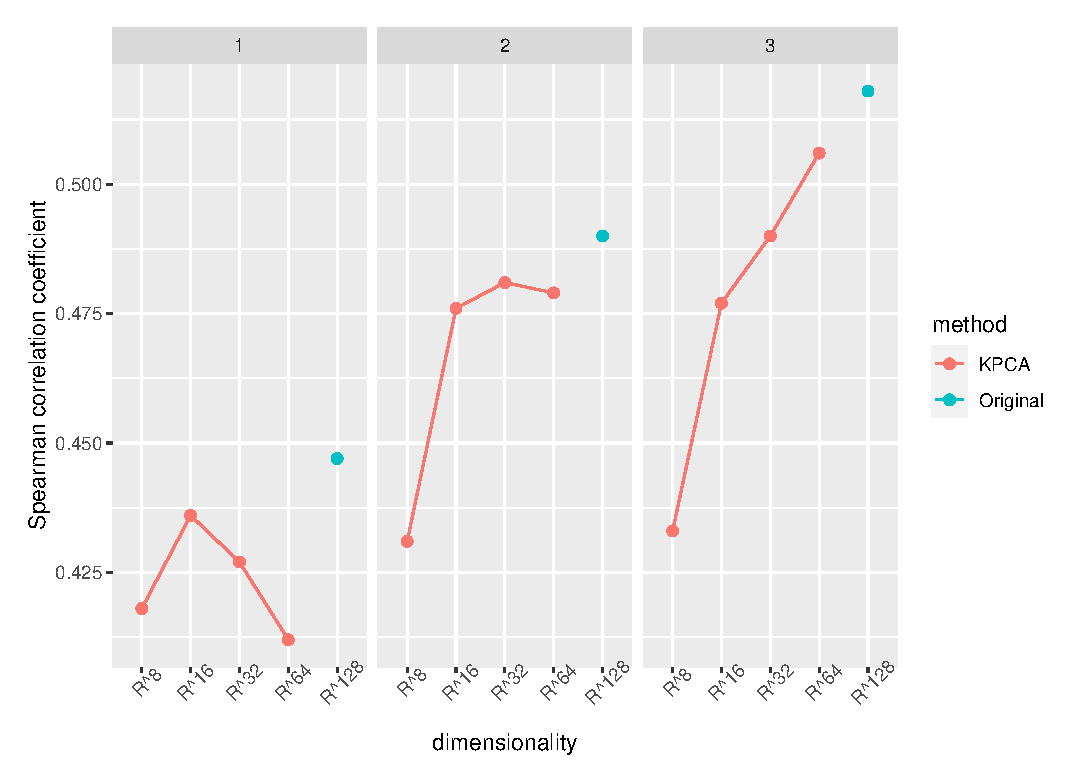
\includegraphics[width=12cm,height=7cm]{./Figures/spear_post.eps}
\caption{\textit{ex-post} KPCA: \textbf{Spearman correlation coefficient} of KPCA embeddings and original embeddings word2vec with state-of-the-art embeddings, for 1, 2, and 3 epochs. Higher is better.} 
\label{fig:spear_post}
\end{figure}




